\section{Tests, Fehlervermeidung und Qualitätssicherung}\label{sec:Testing und Debugging}

%% Einleitung %(
Dieser Abschnitt widmet sich dem Thema der Testverfahren in Softwareprojekten mit dem Schwerpunkt auf dem entwickelten JSF-Projekt 'KuWaSys'.
Zuerst sollen die allgemein geltenden Grundlagen angesprochen werden, darauf aufbauend werden die im Projekt verwendeten Testverfahren näher erläutert. 

Tests lassen sich in der Softwareentwicklung nach ihrer Art und Weise klassifizieren.
Auf der einen Seite steht die konstruktive Qualitätssicherung auf der anderen Seite die analytische.
(Vrgl. \cite{RaM-ST}, 25) 

Zu den konstruktiven Qualitätssicherungsmaßnahmen zählen Durchführungen während des Entwicklungsprozesses selbst:
\begin{itemize}
  \item Checklisten
  \item Programmier-Guidelines
  \item Templates
\end{itemize}

Die analytischen Qualitätssicherung, zu welcher Tests am Produkt gehören, können in zwei verschiedene Testverfahren eingeteilt werden. Hierbei handelt es sich um statische und dynamische Tests.
Verfahren, die hierzu eingesetzt werden, sind für statische Tests:
\begin{itemize}
  \item Statische Analyse
  \item Reviews
\end{itemize}

Im Sinne der statischen Analyse wurden während der Entwicklung folgende Punkte überprüft:
\begin{itemize}
  \item Existenz von Klassen bzw. Methoden
  \item Korrektheit der Scopes der ManagedBeans korrekt
  \item Serialisierbarkeit der ManagedBeans mit dem Scope \texttt{Session} und \texttt{Application}
  \item Konsistenz der Beziehung von MangedBeans und Setter-/Getter-Methoden
\end{itemize}

Und für dynamische Test beispielsweise:
\begin{itemize}
  \item \gls{Blackbox}-Testverfahren
  \item \gls{Whitebox}-Testverfahren
\end{itemize}


Die Planung und Strukturierung der Durchführung von Softwaretests, aber auch die Überlegung von Testfällen, die am System geprüft werden sollen, stellen einen äußerst wichtigen Prozess der Softwareentwicklung dar.
Diese Schritte fließen bestenfalls zu Beginn des Projekts, in der Planungsphase, mit ein.

Als geplante Tests am fertigen System wurden die folgenden vorgesehen und im Checklisten-Verfahren abgearbeitet:
\begin{itemize}
	\item Tests bezüglich der Interaktion am System (mit Testpersonen und deren Feedback)
	\begin{itemize} 
		 \item prüfen der Übersichtlichkeit aller Benutzergruppen
		 \item Kontrolle des Seitenaufbaus und der Strukturierung für effizientes Arbeiten
	\end{itemize}
	\item Testeingaben in Textfelder
	\begin{itemize} 
		 \item Tests der Schnittstellen und der übergebenen Parameter nach Datentyp
		 \item Abklärung von eventuellen Encoding-Problemen
	\end{itemize}
	\item Funktionalitätstests aller Schaltflächen
	\begin{itemize} 
		 \item Absichern von korrekten Systemereignissen bzw. -funktionen
		 \item Kontrolle der übergebenen Werte und Datentypen, um Fehlbelegungen auszuschließen
	\end{itemize}
	\item Konsistenz der Datenbank 
	\begin{itemize} 
		 \item Abfragen mit Hinblick auf Eindeutigkeit, bspw. bei \texttt{UNIQUE-Constraints} sowie \texttt{PRIMARY KEY-} und \texttt{FOREIGN KEY-Constraints}
		 \item Überprüfung der verwendeten Datentypen im System
	\end{itemize}
\end{itemize}

Im Folgenden sollen Tests im Zusammenhang mit der Softwarequalitätssicherung und die Umsetzung im 'KuWaSys' näher betrachtet werden.

Die Qualitätssicherung von Software hat in der heutigen Zeit einen so großen Stellenwert angenommen, dass es mittlerweile sogar ISO-Normen gibt - genauer gesagt die ISO-Norm 9126 - für Qualität in Software. Diese Norm enthält grundlegende Bestimmungen über Effizienz, Funktionalität, Zuverlässigkeit, Benutzbarkeit, Portabilität und Wartbarkeit. 
Die genauen Details der Definitionen werden hier nicht weiter erwähnt, da diese über das Thema der Projektarbeit hinaus gehen würden. Eine gute und vollständige Zusammenfassung der gesamten Norm ist jedoch unter \cite{WikiISO9126} zu finden.

% ISO 9126 MindMap
\begin{figure}[H]
\centering\begin{tikzpicture}[mindmap,
  level 1 concept/.append style={level distance=130,sibling angle=30},
  extra concept/.append style={color=blue!50,text=black}]

\begin{scope}[mindmap, concept color=green, text=white]
\node [concept]at (-2,1) {ISO 9126}[clockwise from=-5]
    child [grow=10] {node [concept] (E) {Effizienz}}
    child {node [concept] (F) {Funktionali-tät}}
    child [grow=240] {node [concept] (E) {Zuverläsig-keit}}
    child [grow=110] {node [concept] (B) {Benutzbar-keit}}
    child [grow=60] {node [concept] (P) {Portabilität}}
    child [grow=280] {node [concept] (W) {Wartbarkeit}};
\end{scope}
\end{tikzpicture}
\caption[\textbf{ISO Norm 9126}]{ISO Norm 9126}
\label{fig:Projekt_Mindmap}
\end{figure}
%)

%% Test/Qualität im Projekt %(
Grundsätzlich wurden allgemein gültige Richtlinien und Code-Konventionen von JSF im Projekt umgesetzt. Dies erhöht die Übersichtlichkeit des gesamten Projekts und wirkt sich positiv auf die kooperierende Entwicklung aus. Dadurch werden gleichermaßen qualitätsichernde Maßnahmen ergriffen, wie auch Fehleranfälligkeiten minimiert.  

Das Benutzen von Templates, welche während der Implementierungsphase eingesetzt wurden, stellt ebenfalls eine Technik dar, die zur Fehlervermeidung beiträgt. Das verwendete Design des 'KuWaSys' musste somit nur einmal definiert und getestet werden und konnte anschließend beliebig oft weiterverwendet werden, ohne dabei das Risiko eingehen zu müssen, dass das Design inkonsistent wird oder dass sich neue Fehler im Projekt einschleichen könnten. 

Um Laufzeittests durchzuführen, wurden FacesMessages über den entsprechenden Import der Klasse \texttt{javax.faces.application.FacesMessage} benutzt, die gleichzeitig die Fehleranalyse mithilfe der Konsole erleichtern.
Ein Beispiel solcher Messages ist in \prettyref{lst:FacesMessages} dargestellt. Im Falle eines Fehlers würde der ausgeführte \texttt{Catch}-Block über den benutzerdefinierten FacesMessages-Befehl eine Ausgabe produzieren.
Nebenbei sei noch eine weitere Besonderheit in JSF angemerkt:
Während der Status 'Development' im  Projekt steht, welcher in der \texttt{pom.xml} festgelegt wird, werden Fehler für bestimmte Funktionen automatisch ausgegeben. Dies ist vor allem bei einem Release zu beachten und vorher abzuändern.

%% Listing: FacesMessages
	\lstinputlisting[label={lst:FacesMessages},
	caption={Debugging mit FacesMessages},
	frame=tlbr, 
	language=java, 
	breaklines=true, 
	numbers=left, 
	numberstyle=\tiny, 
	stepnumber=1, 
	numbersep=5pt, 
	basicstyle=\small\ttfamily,
	showstringspaces=true,
	keywordstyle=\bfseries\color{lila}, 
	tabsize=2,
	backgroundcolor=\color{lightgrey}]{listings/FacesMessages.java}
	
Wie in der folgenden \prettyref{figmin:SchulerImportieren_KuWaSys} zu erkennen ist, wird die Message während der Laufzeit ausgeführt, wie bei diesem missglückten Datei-Upload.

% Kurs anlegen
\begin{figure}[H]
 \begin{center}
   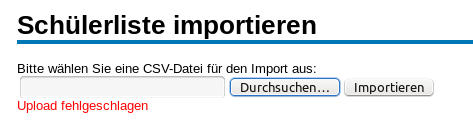
\includegraphics[scale=0.8]{img/SchulerImportieren_KuWaSys.png}
 \end{center}
 \caption[\textbf{KuWaSys: Datei-Upload Fehler beim Schüler Importieren}]{KuWaSys: Datei-Upload Fehler beim Schüler Importieren}
 \label{figmin:SchulerImportieren_KuWaSys}
 \label{fig:SchulerImportieren_KuWaSys}
\end{figure}

Diese Tests erwiesen sich bei Datenbankabfragen als sehr hilfreich, da nicht erst aufwändige Oberflächen umgesetzt werden müssen, um Fehler zu erkennen, sondern Daten sofort auf ihre Richtigkeit hin geprüft werden können.
Diese Fehler sind gleich zu Beginn der Implementierung aufgefallen, da es sich hier vor allem um Fehler handelt, die während der Modellierungs- bzw. Designphase entstanden sind. Diese Fehler sind mit FacesMessages relativ schnell auszumachen und ebenso schnell korrigiert. Beispiele solcher Fehler sind:
\begin{itemize}
  \item falsche Überlegungen zu den Datentypen in der \ac{DB}
  \item schlecht definierte Schnittstellen
  \item Inkonsistenz im Design 
\end{itemize}

Eine weitere Möglichkeit, Fehler in einer Webapplikation zu entdecken, ist das Benutzen von selbstdefinierten Server-Logs.
Hierzu wurde von uns die Klasse \texttt{import java.util.logging.Logger} verwendet. Der \prettyref{lst:Logger}, zeigt wie beispielsweise ein \texttt{Catch}-Block  mitgeloggt werden kann.

%% Listing: Logging
	\lstinputlisting[label={lst:Logger},
	caption={Server-Logging in JSF},
	frame=tlbr, 
	language=java, 
	breaklines=true, 
	numbers=left, 
	numberstyle=\tiny, 
	stepnumber=1, 
	numbersep=5pt, 
	basicstyle=\small\ttfamily,
	showstringspaces=true,
	keywordstyle=\bfseries\color{lila}, 
	tabsize=2,
	backgroundcolor=\color{lightgrey}]{listings/Logger.java}

Da ständig auf einem aktiven System entwickelt und getestet wurde, konnten Tester aus dem Umfeld der Schule für diesen Zweck eingesetzt werden.
Dies erwies sich vor allem beim Entwickeln des Oberflächendesigns als Vorteil. Es konnten Wünsche von Lehrern und Schülern direkt berücksichtigt und umgesetzt werden.
Hier bekommen besonders Checklisten und Reviews einen hohen Stellenwert. Nur durch regelmäßige gemeinsame Treffen konnten Projekttermine (neu-)definiert werden.

Im Hinblick auf die vorher besprochene ISO-Norm 9126 erfüllt das Kurswahlsystem alle Bestimmungen. Jedoch muss fairnesshalber dazu gesagt werden, dass Dinge wie Effizienz in Software nie mit einem genauen Maß gemessen werden kann, da viele Faktoren eine Rolle spielen.
Zum Beispiel müssen bei gewissen Datenstrukturen Laufzeiteinschränkungen in Kauf genommen werden, wenn sich dadurch die Darstellung effizienter umsetzen lässt. Andererseits können natürlich schneller Datenstrukturen oder Algorithmen in einer viel langsameren Darstellung resultieren.
Dasselbe gilt für die Zuverlässigkeit. Natürlich ist das Kurswahlsystem so entworfen worden, dass die Erreichbarkeit und Nutzbarkeit jederzeit gegeben ist. Aber auch hier unterliegt das System mehreren außenstehenden Faktoren, auf die ein Entwickler niemals Einfluss nehmen kann.
%)

%% JSFUnit %(
Selbstverständlich können für den Java Server Faces Standard auch Tests implementiert werden. Diese werden für gewöhnlich bei den dynamischen Test angesiedelt. Von uns wurden keine speziellen Frameworks zur Realisierung von Tests verwendet. Vollständigkeitshalber soll allerdings einer der interessantesten Vertreter von Testinstrumenten für JSF erwähnt werden:

Hierbei handelt es sich um \gls{JSFUnit}, welches auf dem bekannten JAVA-Testframework \gls{JUnit} aufbaut. Tests können hierzu über die JSFUnit-Konsole oder durch den Aufruf einer Testseite ausgeführt werden. Testmöglichkeiten sind Wert- und Zustandsänderungen in ManagedBeans, setzen von Navigationszielen oder über FacesMessages.
Eine besondere Art der Tests sind die 'Acrylic Box'-Testings. Diese verbinden Whitebox und Blackbox-Testverfahren und werden bei den dynamischen Tests eingestuft.
Nähere Informationen sind unter \cite{JSFUnit01} zu finden.
%)

Zuletzt soll noch hinzugefügt werden, dass auch ausführliche Tests keine Garantie auf eine vollständige Fehlerfreiheit geben.
Allerdings helfen Tests, die Fehler möglichst gering zu halten und steigern die Qualität der Software um ein gewisses Maß.
Obwohl das Projekt ausführlichst getestet wurde, kann es dennoch nicht ausgeschlossen werden, dass noch einige existieren. 
